\section{Interface}
\label{sec:interface-ssa}

While the core code-base has been designed and implemented
  to be easily accessible to those who wish to use it directly or extend it,
  the expected everyday interface to this project is
  the graphical tool presented below.
It fully supports the creation and documentation of
  self-stabilizing algorithms,
  rules,
  predicates,
  and moves
  using a combination of textual and graphical interfaces.
Since the bundle format is self-contained,
  all of these objects \Dash
  predicates, moves, and algorithms \Dash
  can be saved and distributed to colleagues
  that are using the same or derivative software.

\subsection{Predicates and Moves}
As reflected in the logical representation
  (see~\autoref{sec:logic-repr:self-stab-algor}),
  self-stabilizing algorithms persist as a collection
  of predicates and moves.
As such, this tool supports the convenient creation of these basic components.

Predicates and moves can be created using the graphical interface,
  but it should be noted that the \emph{definition} of these is left
  as plain-text input.
(See also~\autoref{task:gui-syntax-highlighting} and~\autoref{task:gui-definition-wrapping}.)
(This definition will be written verbatim to disk;
  see \autoref{sec:logic-repr:predicate-move}.)
To create them, navigate to the \ifacefield{Predicates} or \ifacefield{Moves} tabs
  and click the "add" button beneath the list on the far left
  (\autoref{fig:iface:create-pred}).
This will add an empty item \Dash in this case, a predicate \Dash to the list.
Editing its \ifacefield{Name} field will update its name in the list accordingly.
Fill in the \ifacefield{Author}, \ifacefield{Date},
  and \ifacefield{\TeX} fields as appropriate.

When you are ready to provide a definition,
  click the ellipsis ("...") next to the \ifacefield{File} field.
This will present you with a modal dialog within which to provide
  the technical definition for whatever has been created.
The definition must be in Python~3 syntax~\autocite{python3:ref}.
When the definition window opens, you will be presented with
  a short definition of the active variables and their format \Dash
  along with example uses \Dash
  as a comment.
(This can remain as part of the file if you wish.)
Click \ifacefield{OK} to save the file.
\begin{figure}
  \centering
  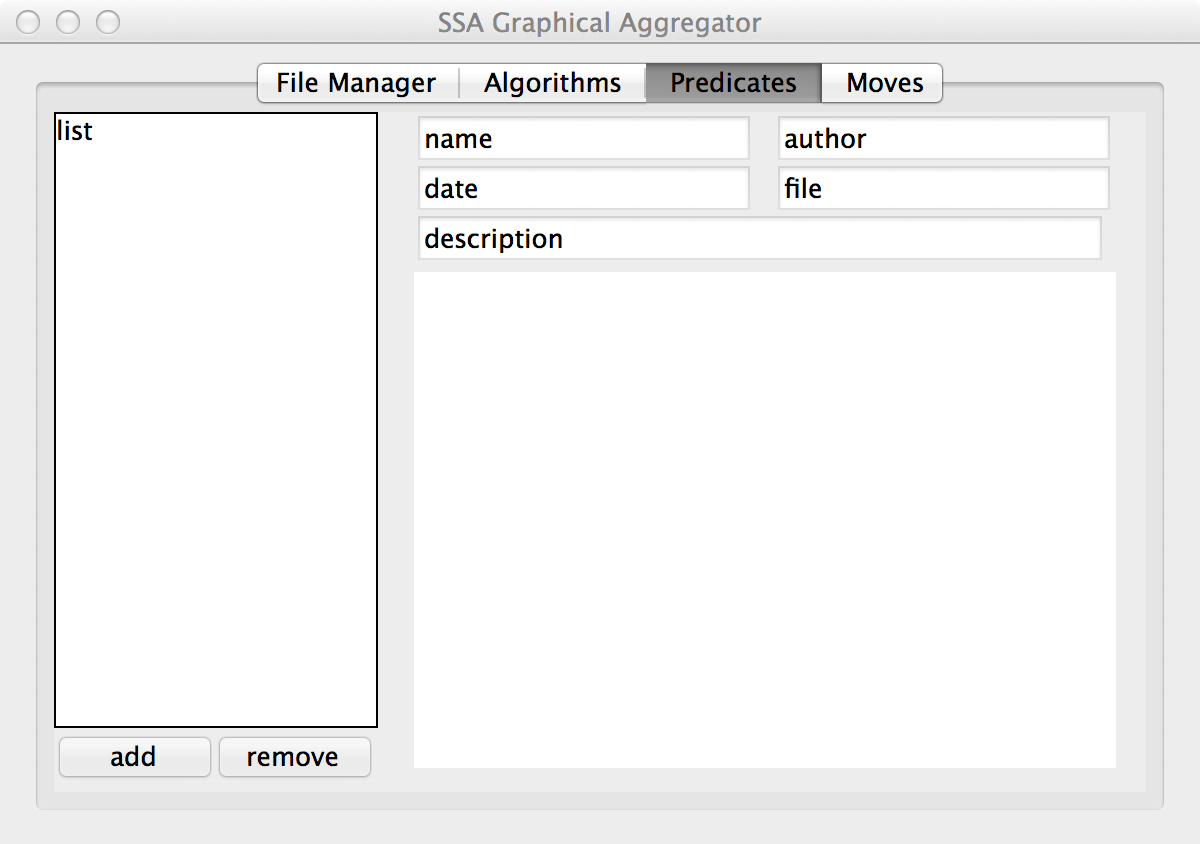
\includegraphics[width=\textwidth]{predicate-move}
  \caption{The predicate\slash move creation screen.}
  \label{fig:iface:pred-screen}
\end{figure}
\begin{figure}
  \centering
\begin{lstlisting}
# This is the definition of a predicate of a self-stabilizing algorithm.
# What follows is the body of a function with the signature given below:
#
#     def privilege(self, v, N)
#
# where `v` is a node (as a dictionary) and `N` is the open neighborhood
# of `v` as a list of dictionaries.

if not v['marked']:
    return False
for neighbor in N:
    if neighbor['marked']:
        return False
return True
\end{lstlisting}
  \caption{When creating an entirely new predicate or move,
    you are presented with a helpful template to start working from.}
  \label{fig:iface:create-pred}
\end{figure}
\begin{warning}
  When you have finished editing the definition for a predicate or move,
    the file is immediately written to disk.
  This action cannot be undone and is unaffected by the \menu{File Manager > Save Bundle} operation.
  This can be mitigated by~\autoref{task:temp-files}.
\end{warning}

\subsection{Documentation}
All entities \Dash predicates, moves, rules, and algorithms \Dash support documentation in various manifestations.
In the graphical interface, these fields include the author,
  a name,\footnote{Required and must be unique.  See~\autoref{sec:bundle-descr-docum}.}
  a description, and \TeX nical documentation.
\paragraph{\TeX nical documentation}
When exporting an algorithm as a PDF (processed via \TeX\slash\TikZ),\footnote{%
  Not yet supported via the graphical interface.
  See~\autoref{task:texport}.}
  the \TeX nical documentation for each entity is given special treatment.
As bundles should be self-sufficient,
  there is an easy syntax to use to denote the properties of a node.
Considering \Algorithm{IndSet}, the quality of being \enquote*{in the set}
  may be denoted as \texttt{\QuoteLiteral{marked}(n) = 1}.
Note the literal double quotes (the single character \texttt{\char`"}) around the function name;
  in addition to clearly describing the purpose of a value,
  this notation will be replaced as appropriate by
  the more verbose (but correct) "\operatorname{marked}".

It should be noted that {\TeX} export is not yet functional in the core tool;
  this syntax is merely set in place to guide further development.
\todo{Update as necessary}
See~\autoref{task:texport}.
\subsection{Algorithms}

Algorithm assembly is fully supported using the graphical interface.
To create an algorithm, simply click the "add" button
  underneath the list of algorithms to the right.
(This list will be empty in a new bundle.)
Once this has been done, giving the Algorithm a name (via the \ifacefield{Name} field)
  will update its text in the listing accordingly.

The process is similar to add new rules to the algorithm.
To create a new rule, simply press the "add" button under the list of rules.
Give it a predicate via the drop-down (which is populated by the list of predicates in their tab)
  and transfer moves between the master list on the left (similarly populated) and the rule's list on the right
  using the angle bracket buttons (">" and "<") between them.
\begin{figure}
  \centering
  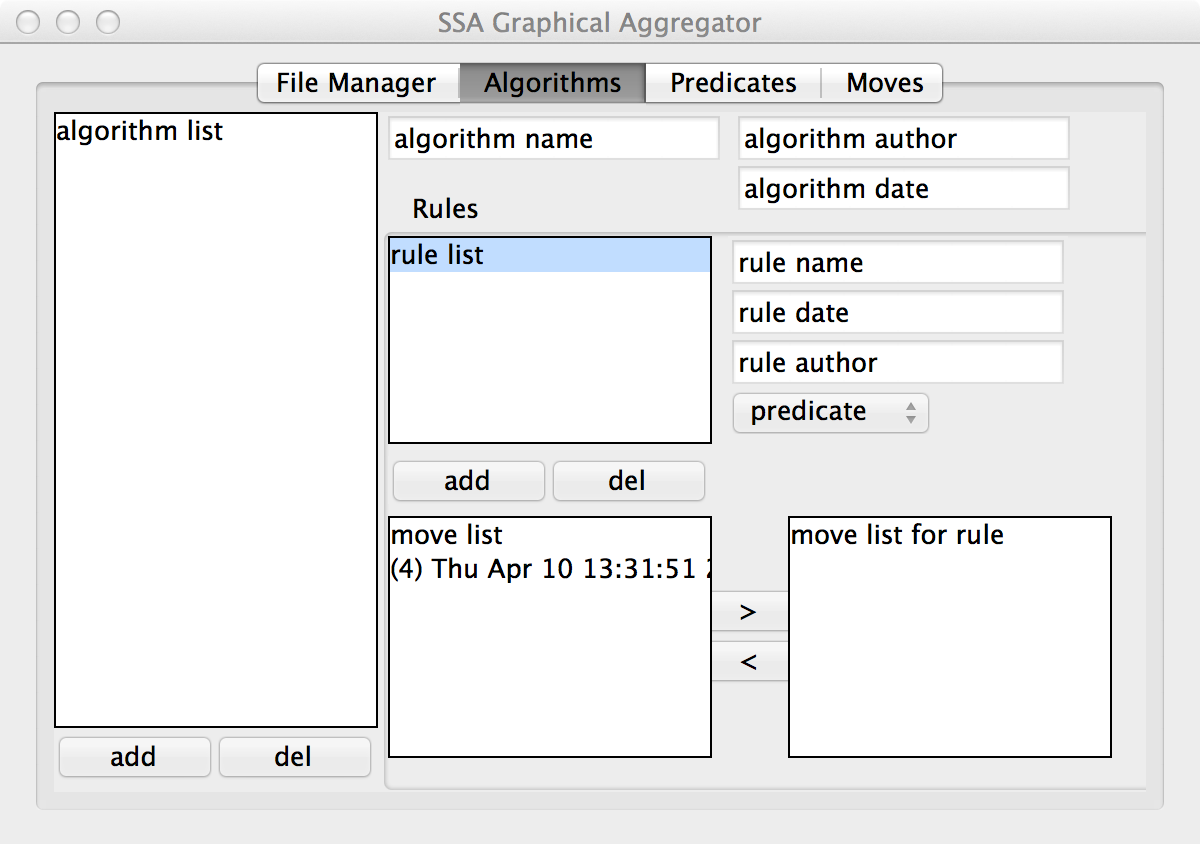
\includegraphics[width=\textwidth]{algorithms}
  \caption{The algorithm assembly screen}
  \label{fig:iface:alg-asm}
\end{figure}

\subsection{Creating, Loading, and Saving}
\label{sec:iface:saving}

To save and load bundles, navigate to \menu{File Manager} tab.
Enter the \emph{full}, \emph{absolute} path of the bundle you wish to load and,
  taking special care not to press \menu{Save Bundle}
  (as this will overwrite it),
  press \menu{Load Bundle}.
Successively loading bundles will aggregate them under a union operation
  to allow for distributed work toward larger and larger bundles.

If you wish to create a \emph{new} bundle, simply press \menu{New Bundle}.
This will clear the interface and allow you to start fresh.

\begin{figure}
  \centering
  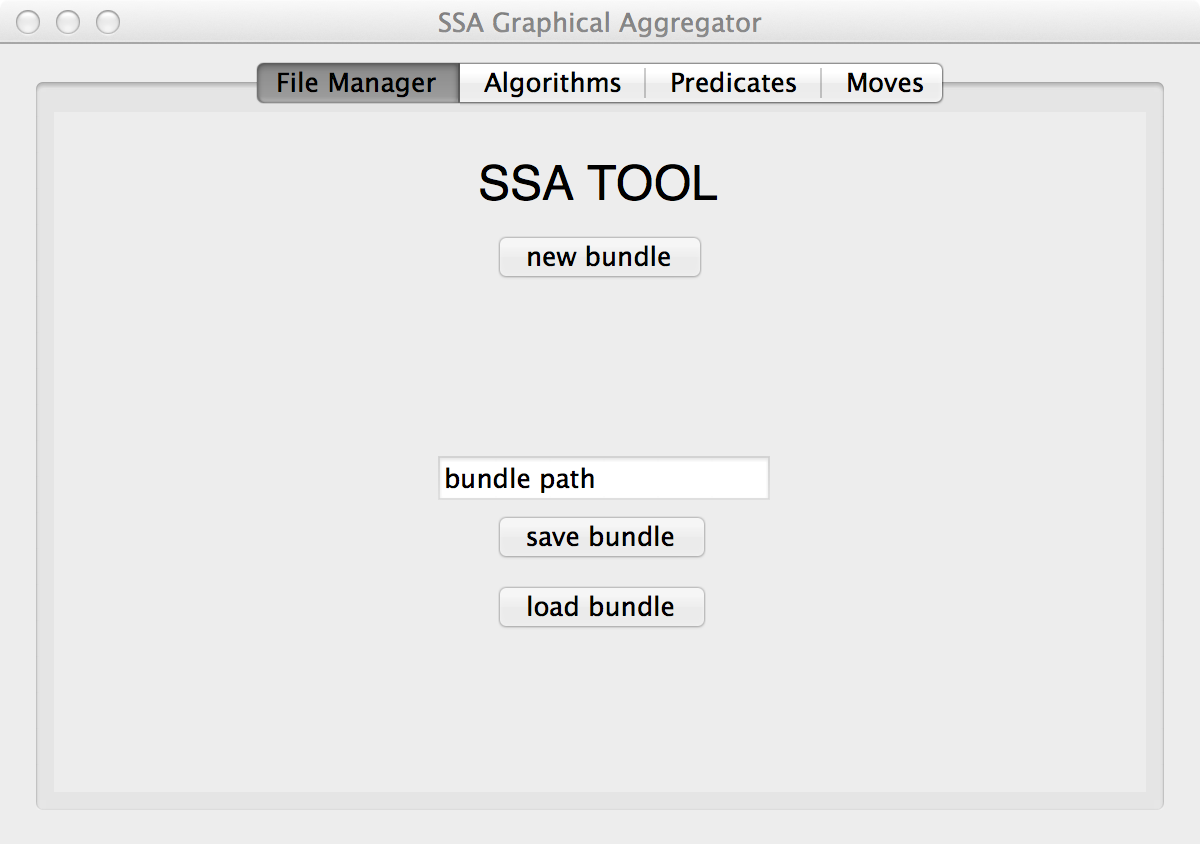
\includegraphics[width=\textwidth]{file-manager}
  \caption{The file management interface}
  \label{fig:iface:fmgr}
\end{figure}

%%% Local Variables: 
%%% mode: latex
%%% TeX-master: "../smp.tex"
%%% reftex-cite-format: "\\autocite{%l}" 
%%% TeX-PDF-mode: t 
%%% TeX-command-default: "arara"
%%% TeX-engine: xetex
%%% End: 
